\documentclass[9pt,twocolumn,twoside]{../../styles/osajnl}
\usepackage{fancyvrb}
\journal{i524} 

\title{Aviation Data Analysis Using Apache Pig}

\author[1*]{Harshit Krishnakumar}
\author[2]{Karthik Anbazhagan}

\affil[1]{School of Informatics and Computing, Bloomington, IN 47408, U.S.A.}
\affil[2]{School of Informatics and Computing, Bloomington, IN 47408, U.S.A.}

\affil[*]{Corresponding authors: harkrish@iu.edu, kartanba@iu.edu}

\dates{Project-002, \today}

\ociscodes{big data, Apache Pig, Apache Hadoop, Chameleon Cloud, Avaiation Analysis}

% replace this with your url in github/gitlab
\doi{\url{https://github.com/cloudmesh/sp17-i524/blob/master/project/S17-IR-P002/report/report.pdf}}


\begin{abstract}
Data science is a challenging field which gives actionable insights into data, enabling businesses to take calculated decisions. Big data techniques help and accelerate the analysis of data in real time. Big Data can be used to monitor things as diverse as flight data, traffic data, and financial transactions. With huge increase in the volume of air travel and drastic weather changes, flights delays and cancellation are on the rise. This project aims at tracking the aviation data and providing a list of the busiest airports by total flight traffic across the US. The system has been deployed in chameleon cloud platform. Apache Pig deployed on a Hadoop cluster is used to join multiple features across massive datasets to query and analyse the data across a Distributed File System.\\
\end{abstract}

\setboolean{displaycopyright}{true}

\begin{document}

\flushbottom % Makes all text pages the same height

\maketitle % Print the title and abstract box

\tableofcontents % Print the contents section
\maketitle

\section{Introduction}
Air travel is getting increasingly popular with the airlines providing cheaper fares and better services \cite{www-aviation-price}. However, owing to the increased congestion in traffic during festive season and ever fluctuating weather conditions, there are cancellations and delays to the flights. Cancellations tend to be costly for both passengers and the airline companies and pose difficulties for the customers who might have appointments or connecting flights. According to new Department of Transportation filings \cite{www-airline}, the resulting change fees and cancellation penalties passengers end up paying up to a whopping \$2 billion a year. 

With the increasing availability of data and improvement technology, there is growth in the area of big data and computing \cite{www-hdfs-arch}. There has been development of new tools and frameworks to efficiently process large amounts of data. These tools rapidly process data and execute complex parallel algorithms while automatically splitting the the work across a set of available nodes. Earlier data processing applications could not handle the high volume, velocity, and variety of big data. This is the data which is difficult to handle in conventional data analytics. Big Data is now being used to monitor things as diverse as flight data \cite{www-aviation}, traffic data, and financial transactions. The challenge of Big Data is how to use it to create something that is value to the user. How to gather it, store it, process it and analyze it to turn the raw data information to support decision making. This paper aims to leverage big data by deploying a Hadoop cluster and running an analysis across large datasets containing airline cancellations and delays details using Pig Scripts and provide insights almost in real-time. 

Hadoop allows to store and process Big Data in a distributed environment across group of computers. It is intended to scale up starting with a single machines and will be scaled to many machines. In our analysis we benchmark the performance of the clusters for various data sizes and cluster configurations. We utilize Chameleon cloud to run the Hadoop cluster and perform our benchmark.

\section{Architecture}
\subsection{Cloudmesh Client}
Cloudmesh client is a lightweight cloud client to manage virtual clusters. It enables users to access multiple cloud environments from command shell and commandline. Cloudmesh client allows to easily manage virtual machines, containers, HPC tasks, through a convenient client and API. It is a client based toolkit that is installed and run on the users computers. The installation has been done on Ubuntu 16.04 for this project. It has a layered architecture that allows easy development of new features. A resource abstraction layer allows the integration of a multitude of resources spanning HPC, Containers, and Cloud resources. 


Using Cloudmesh Client's "cm define" and "cm deploy" command with the right configurations, it is possible to define and create a multi node cluster and install Hadoop with addons. The architecture of Cloudmesh Client makes the deployment of clusters simple from Ubuntu shell with basic commands. 

\subsection{Ansible}
Ansible is an open-source automation tool that automates software provisioning, configuration management, and application deployment. Once Ansible gets installed on a control node, which is an agentless architecture \cite{wiki-ansible}, it connects to a managed node through the default OpenSSH connection type. The architecture of Ansible is shown in \ref{fig:ansible}. As with most configuration management softwares, Ansible distinguishes two types of servers: controlling machines and nodes. First, there is a single controlling machine which is where orchestration begins. Nodes are managed by a controlling machine over SSH. The controlling machine describes the location of nodes through its inventory.


Ansible manages machines in an agent-less manner, it doesn't requires any software to be installed on the remote machines to make them manageable. By default is manages remote machines over SSH or WinRM \cite{www-ansible}, which are natively present on those platforms. These modules are temporarily stored in the nodes and communicate with the controlling machine through a JSON protocol over the standard. Ansible is decentralized, if needed, Ansible can easily connect with Kerberos, LDAP, and other centralized authentication management systems.




The design goals of Ansible includes consistency, high reliability, low learning curve, security and to be minimalistic in nature. Ansible doesn't require dedicated users or credentials - it respects the credentials that the user supplies when running Ansible. Similarly, Ansible does not require administrator access, it leverages sudo, su, and other privilege escalation methods on request when necessary \cite{git-ansible}.

\begin{figure}[htbp]
\centering
\fbox{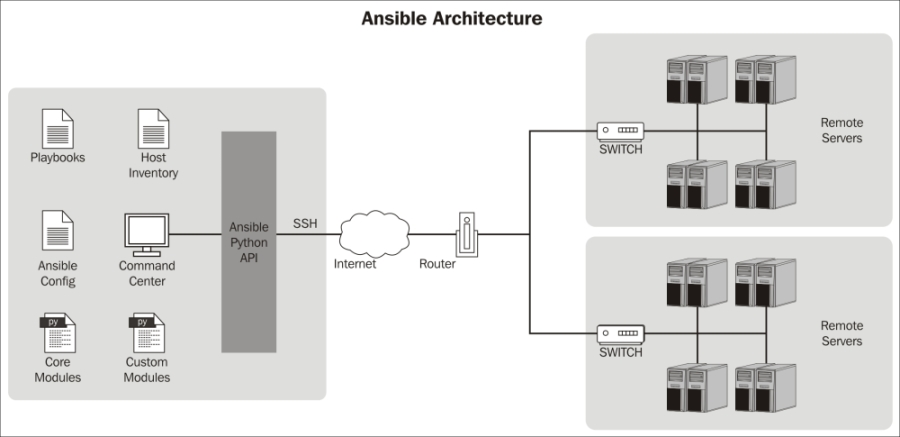
\includegraphics[width=\linewidth]{images/ansible.jpg}}
\caption{Architecture of Ansible \cite{www-ansible-fig}}
\label{fig:ansible}
\end{figure}


The functioning of Ansible allows users to define the ip address of namenode in the hosts file, and give the required instructions in .yml file. The configuration yaml file is called Ansible Playbook, and can be run to perform all the tasks listed in it on all the servers mentioned in the hosts file. This way Ansible makes handling multiple virtual machines simple by iteratively performing a set of tasks on all the hosts. In the hosts file, individual host name can be grouped together to form host groups, which can be called for advanced installations. Ansible also has options to assign roles to perform a specified set of tasks, its own version of modularization. There are options to use variables in the playbook. The current project uses Ansible to handle the movement of files between servers, and to run Shell commands on Hadoop namenode. 

\subsection{Chameleon Cloud}
Chameleon Cloud is an open source large scale cloud platform available for the research community. The current commercial cloud platforms are mostly inaccessible for the student and research community. Chameleon project was created with funding from National Science Foundation and has 650 multi-core cloud nodes, 5PB of total disk space, and ability to leverage 100 Gbps connection between the sites. Chameleon cloud enables users to experiment on transformative concepts in deeply programmable cloud services, design, and core technologies on problems ranging from the creation of Software as a Service to kernel support for virtualization. However, Chameleon cloud  of supported research includes many other areas such as developing Platforms as a Service, creating new and optimizing existing Infrastructure as a Service components, investigating software-defined networking, and optimizing virtualization technologies. \cite{www-cham-cloud}

The current project uses Chameleon Cloud instance created for the Big Data class at Indiana University. The current instance allows cloud created in three flavors - small, medium and large. Chameleon Cloud allows users to create any number of virtual machines with the required flavor, and allows to assign floating public IPs to be accessible from the outside. Each of the virtual machines can be created using any Operating System, and the current project uses Ubuntu14.04 version installed on Chameleon Cloud.

\subsection{Hadoop}
Apache Hadoop is an open-source software framework for storage and large-scale processing of data-sets on clusters of commodity hardware. Hadoop is written in Java, and it allows parallal processing of large datasets. Hadoop has four main components \cite{www-had-tut-point}:

\begin{enumerate}
    \item \textbf{Hadoop Common:} These are the basic Java libraries and configuration files required for Hadoop to run
    \item \textbf{Hadoop YARN:} Yarn is Hadoop's resourse navigator. It is used for resource management and job scheduling
    \item \textbf{HDFS:} The Distributed File System is Hadoop's data storage. It distributes the data across Hadoop cluster
    \item \textbf{Hadoop MapReduce:}It is a Yarn based system used to ro distribute Hadoop jobs across cluster
    \end{enumerate}

\begin{figure}[htbp]
\centering
\fbox{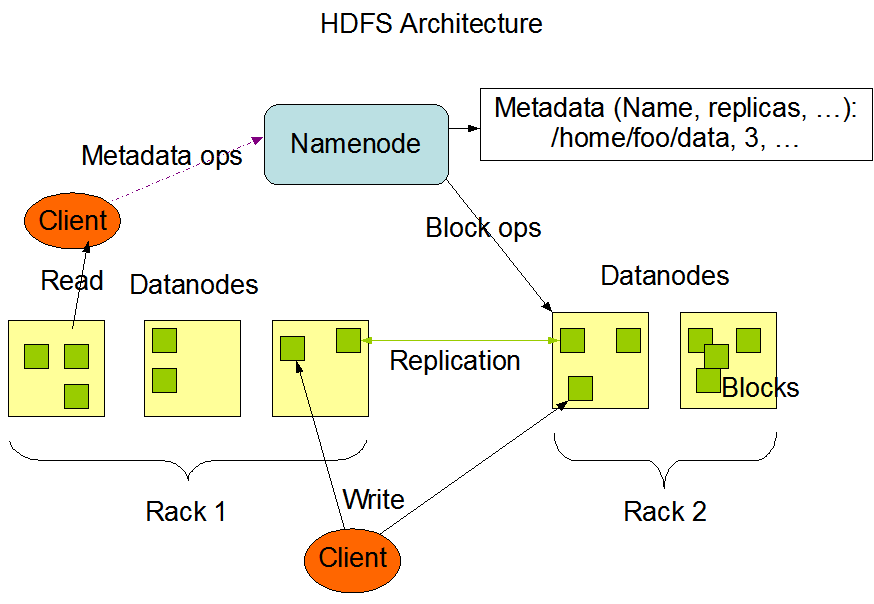
\includegraphics[width=\linewidth]{images/HDFS.png}}
\caption{Architecture of Hadoop \cite{www-hdfs-fig}}
\label{fig:ansible}
\end{figure}

\subsubsection{HDFS}
HDFS is a fault-tolerant system designed to be deployed on low-cost hardware. HDFS works well with large data sets and provides high throughput access to application data.
A typical file in HDFS is in gigabytes to terabytes in size.  HDFS has a master-slave architecture. A typical HDFS cluster consists of a single NameNode, a master server that manages the files system, a number of DataNodes which manages the storage attached to the node they run on. Internally, a file is split into multiple blocks and these blocks are stored in a set of DataNodes. The NameNode executes file system namespace operations like opening, closing, and renaming files and directories. It also determines the mapping of blocks to DataNodes. The DataNodes also perform block creation, deletion, and replication upon instruction from the NameNode.

The NameNode and DataNode are pieces of software designed to run on any machine. HDFS is built using the Java language. Any machine that supports Java can deploy HDFS. A deployement takes place in such a manner that one machine runs the NameNode software and each of the other machines runs one instance of the DataNode software. The presence of a NameNode is a must and the presence of a single NameNode in a cluster greatly simplifies the architecture of the system. The system is designed in such a way that user data never flows through the NameNode.

\subsubsection{MapReduce}
Hadoop enable distributed processing of massive structured/unstructured data across multiple commodity computers where each node contains it own data storage. This programming model of parallel processing and assimilation is the MapReduce program. MapReduce hsa two main functions - a Mapper class and a Reduce class. MapReduce serves two essential functions: It parcels out work to various nodes within the cluster or map, and it organizes and reduces the results from each node into a cohesive answer to a query. \\

MapReduce is composed of several components, including:
\begin{itemize}
    \item JobTracker: the master node that manages all jobs and resources in a cluster
    \item TaskTrackers: agents deployed to each machine in the cluster to run the map and reduce tasks
    \item JobHistoryServer: a component that tracks completed jobs, and is typically deployed as a separate function or with JobTracker

\end{itemize}
    



\subsection{PIG}
PIG uses Pig Latin to analyse data in Hadoop. To perform data analysis, programmers need to write a Pig script using the Pig Latin language. Pig converts these scripts into multiple MapReduce jobs. There are various components in the Apache Pig framework:
\begin{itemize}
    \item Parser: It checks the syntax of the script and displays the output (logical statements) in the form of DAG, 
    \item Optimizer: performs logical optimizations such as such as projection and pushdown, 
    \item Compiler: complies the logical output into series of MapReduce jobs, 
    \item Execution engine: executes the MapReduce jobs are submitted to Hadoop in a sorted order.
\end{itemize}

\begin{figure}[htbp]
\centering
\fbox{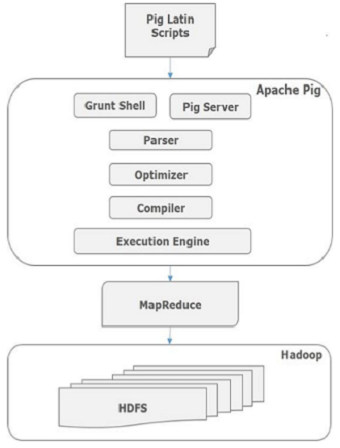
\includegraphics[width=\linewidth]{images/pig.png}}
\caption{Architecture of PIG \cite{www-pig-fig}}
\label{fig:ansible}
\end{figure}


\section{Work flow}

\subsection{Hadoop Deployment}
The deployment was done from an Ubuntu14.04 instance running on Oracle Virtual Box. Hadoop instance with three nodes was deployed on Chameleon cloud using Cloudmesh Client was used to automatically create the cluster and deploy Hadoop software with Pig and Spark add-ons. Three virtual machines with Ubuntu14.04 version were installed on Chameleon Cloud, and Hadoop along with Pig and Spark add-ons was deployed to the clouds with one name node and two data nodes. 

\subsection{Cluster Configurations}
Hadoop was deployed on a cluster with three nodes. Three virtual machines were created on Chameleon Cloud for this purpose, with one instance as namenode (master) and rest of the instances as datanodes (slaves). All the three virtual machines were created with Ubuntu14.04 OS. Each of the vms had 20 GB space, with 2GB ram and one CPU. This configuration is called the "small" flavour in Chameleon Cloud. Each vm was assigned a separate floating public IP which could be used to SSH and connect. 

\subsection{Ansible Playbook}
Ansible was installed in the oracle virtual box and configured to automatically perform file transfers and to run Pig code on the cluster. All our interactions are with the namenode of  Hadoop, so the public IP of the namenode of our installation was given in the hosts file of Ansible for all purposes. 

Five Ansible Playbooks were setup, each with the following purposes:

\begin{enumerate}
    \item Transfer data and Pig Script files to namenode from local location
    \item Transfer data files to hdfs location on namenode using \textit{hdfs dfs} command
    \item Run pig code using \textit{pig <any\_pig\_script>} shell command on the name node
    \item Transfer the output files from hdfs back to namenode 
    \item Transfer output files to local location
\end{enumerate}

Each of these would run on the locations mentioned in hosts file on usernames CC and hadoop, which were the default users created by cloudmesh client. 


\section{Airline Analysis}
\subsection{Datasets}
The current project focuses on analysing flight cancellations and delays data to find trends. The dataset is taken from the US Department of Transportation's Bureau of Statistics \cite{www-rita}. Their website releases monthly air travel statistics and summary report of all the flights information of previous month. Along with this report, they release the raw data which is openly available to be downloaded and analysed. The two datasets we use are taken from the raw data provided in the website. A brief description about the datasets is given below.
\begin{enumerate}
    \item \textbf{Delayed Flights} contains information about all the cancelled or delayed flights ranging across the years 1987 to 2008. It has 29 columns which are described in the Table 1.
    
    \begin{table}
    \begin{tabular}{|c|c|}
        \hline
        \textbf{Column Name} & \textbf{Description} \\ \hline
        Year & 1987-2008  \\ \hline
        Month & 1-12  \\ \hline
        DayofMonth & 1-31  \\ \hline
        DayOfWeek & 1 (Monday) - 7 (Sunday)  \\ \hline
        DepTime & actual departure time   \\ \hline    
        CRSDepTime & scheduled departure time  \\ \hline
        ArrTime & actual arrival time \\ \hline
        CRSArrTime & scheduled arrival time  \\ \hline
        UniqueCarrier & unique carrier code  \\ \hline
        FlightNum & flight number  \\ \hline
        TailNum & plane tail number  \\ \hline
        ActualElapsedTime & in minutes  \\ \hline
        CRSElapsedTime & in minutes  \\ \hline
        AirTime & in minutes  \\ \hline
        ArrDelay & arrival delay in minutes  \\ \hline
        DepDelay & departure delay in minutes  \\ \hline
        Origin & origin IATA airport code  \\ \hline
        Dest & destination IATA airport code  \\ \hline
        Distance & in miles  \\ \hline
        TaxiIn & taxi in time, in minutes  \\ \hline
        TaxiOut & taxi out time in minutes  \\ \hline
        Cancelled & was the flight cancelled?  \\ \hline
        CancellationCode & reason for cancellation  \\ \hline
        Diverted & 1 = yes, 0 = no  \\ \hline
        CarrierDelay & in minutes  \\ \hline
        WeatherDelay & in minutes  \\ \hline
        NASDelay & in minutes  \\ \hline
        SecurityDelay & in minutes  \\ \hline
        LateAircraftDelay & in minutes  \\ \hline

    \end{tabular}
    \caption{Delayed Flights Column Information}
    \end{table}
    \item \textbf{Airports} is a reference dataset, which gives the airport names and locatons. The column description is shown in the Table 2.
    
    \begin{table}
    \begin{tabular}{|c|c|}
        \hline
        \textbf{Column Name} & \textbf{Description} \\ \hline
        iata & Airport Code  \\ \hline
        airport & Airport Name  \\ \hline
        city & Airport City  \\ \hline
        state & State Code  \\ \hline
        country & Country Code  \\ \hline
        lat & Lattitude  \\ \hline
    long & Longitude  \\ \hline
    \end{tabular}
    \caption{Airports Column Information}
    \end{table}
    
\end{enumerate}
The Delayed Flights dataset is around 250 mb in size and the airports dataset is around 250 kb since it is reference data.
\subsection{Pig Script}
Pig installation runs on the Hadoop hdfs system. The script needed for this analysis was based out of the idea from the blog post written by Sumit Anand \cite{www-acadguild}. It takes the two datasets, performs basic joins, orders the rows and returns top five airports which cause most delays in all the years. This script was run on the namenode on Pig hadoop mode, with the input files given from hdfs dfs locations. This script analyses the data and outputs into hdfs location. The codes are written in Pig Latin language and can be run in Pig grunt shell. 

\section{Benchmarking}
Benchmarking is a process in software development which allows developers to determine the performance of their systems. This can be done for multiple reasons including looking for improvements and future planning. The basic requirements of a benchmark are that the environmental conditions of test should be same each time it is run, and the test should be repeatable. 

The current paper presents multiple levels of benchmarking, starting from the time taken to deploy Hadoop cluster with three nodes, the time taken to move files from local to namenode and hdfs, time taken to run the pig code and time taken to move files from hdfs to namenode and local. Deployment of Hadoop cluster is done using Cloudmesh Client, and the rest of the tasks are done using Ansible. For all Ansibls steps, there are individual playbook files which can be called from separate Ansible commands. Each of these steps has been timed using Ubuntu Shell's "\textit{time}" command. 

Excluding the time taken to download, install and configure Cloudmesh Client, the time taken to create three vms with the "small" configuration, deploy Hadoop with three nodes, Spark and Pig addons is 8 minutes 46 seconds. This deployment was done from Oracle Virtual Box with a ram capacity of 8 GB. 

The experiment was performed on the entire dataset, and the tests were repeated with 50\% and 25\% of the data. The results of the benchmarking tests are given in the tables 3, 4 and 5.

\begin{table}[h!]
\begin{tabular}{|c|c|}
\hline
\textbf{Task} & \textbf{Time Taken} \\ \hline
Copy Data to cloud & 1 min 33 sec  \\ \hline
Copy Data to HDFS & 23 sec  \\ \hline
run pig script & 3min 1 sec  \\ \hline
Copy output to cloud & 25 sec  \\ \hline
Copy output to local & 17 sec  \\ \hline
\end{tabular}
\caption{Benchmark Results for the entire data}
\end{table}

\begin{table}[h!]
\begin{tabular}{|c|c|}
\hline
\textbf{Task} & \textbf{Time Taken} \\ \hline
Copy Data to cloud & 54 sec  \\ \hline
Copy Data to HDFS & 20 sec  \\ \hline
run pig script & 1 min 55 sec  \\ \hline
Copy output to cloud & 24 sec  \\ \hline
Copy output to local & 16 sec  \\ \hline
\end{tabular}
\caption{Benchmark Results for the 50\% of the data}
\end{table}

\begin{table}[h!]
\begin{tabular}{|c|c|}
\hline
\textbf{Task} & \textbf{Time Taken} \\ \hline
Copy Data to cloud & 27 sec  \\ \hline
Copy Data to HDFS & 19 sec  \\ \hline
run pig script & 1 min 6 sec  \\ \hline
Copy output to cloud & 22 sec  \\ \hline
Copy output to local & 17 sec  \\ \hline
\end{tabular}
\caption{Benchmark Results for the 25\% of the data}
\end{table}

\section{Summary}
Airline industry is rapidly growing as the customers who take flights are increasing. Considering this trend, the cancellations and delays come into focus. It is imperative that Big Data technologies are deployed in this sector for quick results. This project aims at using Hadoop and Pig to run a basic analysis on Flight Delays data and benckmark the clouds' performance. 

As we can see from the benchmark results, there is a drastic decrease in the first three steps (copy data to cloud, copy data to hdfs and run pig script) when the input file size is decreased. This is expected since there is less data for Hadoop to crunch. However in each of these cases, the output is top 3 airports, which is a textfile with three records. Thus we do not see much of a change in the time to copy the output (last two steps).

Overall, the time taken to run this entire process starting from copying data to namenode to getting output to local is taking less than 6 minutes for the entire dataset. Keeping in mind that our benchmark was for the "small" flavor of Chameleon Cloud (2GB ram) this is a good score, and if the cluster is vertically or horizontally scaled up, this analysis will yield results quicker. In order to take full advantage of Hadoop's parallel processing capabilities, it would be ideal if the number of nodes in the cluster were increased (horizontal scaling).



\section*{Acknowledgements}

The author thanks Professor Gregor Von Lazewski for providing us with the guidance and topics for the Project. The author also thanks the AIs of Big Data Class for providing the technical
support.


% Bibliography

\bibliography{references}
 
\section*{Author Biographies}
\begingroup
\setlength\intextsep{0pt}
\begin{minipage}[t][3.2cm][t]{1.0\columnwidth} % Adjust height [3.2cm] as required for separation of bio photos.
{\bfseries Harshit Krishnakumar} is pursuing his MSc in Data Science from
Indiana University Bloomington\\
{\bfseries Karthik Anbazhagan} is pursuing his MSc in Data Science from
Indiana University Bloomington
\end{minipage}
\endgroup

\end{document}
